\chapter{Niveau 1 : La Fausse Tombe}
\section{Structure}
Cette section introduit les bases de la conception et exploration de donjon en 7 salles.

Elle est pile de la bonne longueur pour une première session, pourvu que la création de personnages ait été rapide et que vous ayez donné aux PJ une bonne raison d'explorer la tombe.

Elle symbolise la joie de la découverte, le moment où l'on se dit \emph{"Oh ! Je vois !"} et l'anticipation du trésor à venir.

Assurez-vous de féliciter tout joueur parvenant à déduire qu'il s'agit d'une fausse tombe : l'astuce se doit d'être récompensée.
\vfill
\pagebreak
\section{Description}
Décrivez cette zone avec des mots comme "branlant", "décrépi" et "humide".
C'est une vieille cave.
De petites racines blanches pendent du plafond pour venir lécher le sol.
\vfill
\pagebreak

\begin{figure}[hb]
  \centering
  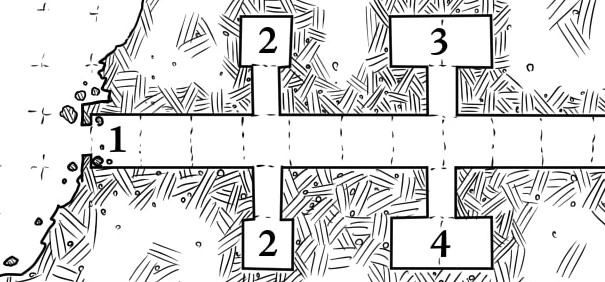
\includegraphics[width=\linewidth]{pics/map_1-4.jpg}
\end{figure}
\subsection{1 : Hall d’Entrée}\label{n1:s1}
\begin{itemize}
  \item 37m de long, sur 3m de large et 3m de haut.
  \item La lumière du soleil en atteint l’extrémité.
  \item Sent la \textbf{poussière}. Plus \textbf{froid} qu’à l’extérieur.
  \item Fines racines au plafond, \textbf{roche taillée grossièrement}
  \item 2 ouvertures de 1.5m de large chaque côté.
  \item Se termine par une porte barrée menant en \textbf{\nameref{n1:s6}}.
\end{itemize}

\subsection{2 : Tombes des Gardes}\label{n1:s2}
\begin{itemize}
  \item Salle de 3m sur 3m, 2.5m de haut
  \item Sent la \textbf{poussière} et le \textbf{vieux bois}, avec un léger \textbf{relent acide}.
  \item Roche taillée grossièrement, 
  \item Fresques de serpents entrelacés.
  \item Un \textbf{cercueil de bois} orné de gravures de scènes de bataille. Renferme :
  \begin{itemize}
    \item Statue de \emph{guerrier} en argile creuse, contient :
    \begin{itemize}
      \item une amulette d’or (10 PO)
      \item un squelette de serpent desséché
    \end{itemize}
    \item \textbf{Piège :} nuage de gaz empoisonné (Sauvegarde Poison ou 1d6 dégâts)
  \end{itemize}
\end{itemize}

\vfill\break
\subsection{3 : Tombe d’Érudit}\label{n1:s3}
\begin{itemize}
  \item Salle de 6m sur 3m, 2.5m de haut
  \item Sent la \textbf{poussière} et le \textbf{tissu putréfié}
  \item Roche taillée grossièrement
  \item Fresques de serpents bondissants.
  \item Un \textbf{cercueil de bois} orné de gravures abstraites, renferme :
  \begin{itemize}
    \item Statue d'\emph{érudit} creuse
    \begin{itemize}
      \item une amulette d’or (10 PO)
      \item un squelette de serpent desséché
    \end{itemize}
    \item Parchemins tombés en poussière
    \item \textbf{Piège :} nuage de gaz empoisonné (Sauvegarde Poison ou 1d6 dégâts)
  \end{itemize}
\end{itemize}

\subsection{4 : Tombe de Sorcier}\label{n1:s4}
\begin{itemize}
  \item Salle de 6m sur 3m, 2.5m de haut
  \item Sent la \textbf{poussière} et le \textbf{tissu putréfié}
  \item Roche taillée grossièrement
  \item Fresques de serpents bondissants.
  \item Un \textbf{cercueil de bois} orné de gravures macabres, renferme :
  \begin{itemize}
    \item Statue de \emph{sorcier} creuse
    \begin{itemize}
      \item une amulette d’or (10 PO)
      \item un squelette de serpent desséché
    \end{itemize}
    \item \textbf{Piège :} nuage de gaz empoisonné (Sauvegarde Poison ou 1d6 dégâts)
    \item Porte un anneau d’argent. Si arraché :
    \begin{itemize}
      \item Brise la statue
      \item Projette le poison
    \end{itemize}
  \end{itemize}
\end{itemize}

\begin{highlight}[Anneau d’argent]
  \begin{itemize}
    \item magique \textbf{et} maudit
    \item Porté au doigt, l’ongle s’allonge et bifurque en deux pointes aiguisées comme des crocs.
    \item Mêmes effet qu'une dague empoisonnée :
    \item Chaque matin  : Sauvegarde contre le poison ou 1d6 dégâts.
    \item Si 6 dégâts :  le doigt tombe et se transforme en serpent.
  \end{itemize}
\end{highlight}

%\begin{highlight}
%\textbf{Leçons :} Les trésors cachés peuvent être magiques, utiles et parfois maudits.
%\end{highlight}

\newpage
\subsection{5 : Porte / Marteau}\label{n1:s5}
Le corridor se termine par une \textbf{porte barrée}.
Deux pieux de fer plantés de chaque côté du chambranle soutiennent une lourde barre de pierre, bloquant l’accès à la salle suivante.

\begin{itemize}
  \item 3 PJ au moins pour la soulever
  \item \textbf{Soulevée :} Piège (Sauvegarde Mort ou 2d6+4 dégâts).
\end{itemize}

\begin{highlight}[Le piège]
  \begin{itemize}
    \item Marteau de pierre bascule du plafond
    \item Remplit \emph{presque} intégralement le couloir
    \item \textbf{\'Eviter :}
    \begin{itemize}
      \item Se plaquer au mur
      \item S'aider d'un autre PJ pour prendre appui : +2 au jet, -2 à l'autre PJ.
    \end{itemize}
    \item \textbf{Détection :}
    \begin{itemize}
      \item Examiner la porte, le plafond
      \item Examiner les pieux : se redressent lentement lorsque la barre est soulevée
    \end{itemize}
    \item \textbf{Désactiver :}
    \begin{itemize}
      \item Replacer la barre
      \item Maintenir les pieux en position basse
      \item Endommager le mécanisme au plafond
    \end{itemize}
  \end{itemize}
\end{highlight}

À moins que quelque chose ne le bloque, le marteau se rétracte lentement dans le plafond.

Il peut être activé à nouveau en abaissant les pieux de fer, à la main ou avec une corde.

L’impact force violemment l’ouverture des portes menant en \textbf{\nameref{n1:s6}}

\subsection{7 : Faux Temple}\label{n1:s7}
\begin{itemize}
  \item Salle de 6m sur 6m, 3m de haut
  \item Sent  fortement le \textbf{moisi},et la \textbf{pierre humide}
  \item \textbf{Statue d’un dieu homme-serpent}.
  \begin{itemize}
    \item Gigantesque, Hideux
  \end{itemize}
  \item Eau suinte du plafond
  \item L'eau a érodé le sol
  \item S'infiltre sous la statue :
  \begin{itemize}
    \item Révèle \textbf{\nameref{n2:s8}} vers le \textbf{\nameref{n2}} du donjon
  \end{itemize}
\end{itemize}
\vfill

\begin{center}
  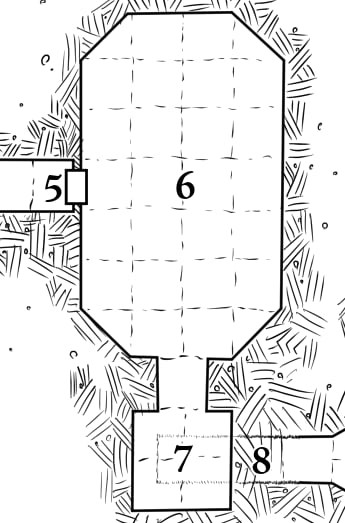
\includegraphics[width=\columnwidth]{pics/map_5-8.jpg}
\end{center}
\subsection{6 : Fausse Tombe Royale}\label{n1:s6}
La chambre funéraire du roi des hommes-serpents et ses deux épouses.
\begin{itemize}
  \item Salle de 12m sur 21m, 2.5m de haut
  \item Sent la \textbf{poussière}, \textbf{l’os} et le \textbf{moisi}
  \item Roche taillée grossièrement
  \item Fresques délitées de paysages.
  \item \textbf{3 cercueils de bois} long du mur nord
  \begin{itemize}
    \item Peints: hommes serpents endormis.
    \item Celui du milieu plus volumineux
    \item Contiennent chacun un \textbf{\nameref{monster:s6}}
    \item Attaquent dès que leur repos est troublé
  \end{itemize}
\end{itemize}



%\begin{highlight}
%\textbf{Leçons :} il y a des passages secrets.
%Ils sont associés aux statues.
%Il pourrait s’agir d’une fausse tombe.
%Tout au long de ce donjon, les statues sont synonymes de passages secrets et de trésors.
%\end{highlight}